%!TEX spellcheck = de
\documentclass[german,notoc,draft]{tudbeamer}%note: when switching to the tud titlestyle, an additional build is needed

%!TEX root = ./main.tex
%!TEX spellcheck = de 
\bibliography{bibliography.bib}

% Einstellungen für Beispielfolien
	% Einpinden des pgf-pie package für Tortendiagramme
	\usepackage{pgf-pie}

	% Ergänzen des Latex-Styles für spezielle hervorhebungen in Listings
	\lstdefinestyle{latex}{
		language=[LaTeX]TeX,
		moredelim=*[s][]{\{}{\}},
		%moredelim=*[s][]{\[}{\]},
		moredelim=*[is][\color{emph2_3}]{*n}{*},
		moretexcs={setDesignImage,frametitle,movie},
		moredelim=*[is][stringstyle]{*s}{*},
		moredelim=*[is][\color{emph2_3}]{*e}{*},
		moredelim=*[s][\color{emph2_4}]{<}{>}
	}

	%Für das Formelbeispiel
	\DeclareMathOperator{\Div}{div}
	\DeclareMathOperator{\Rot}{rot}

%Präambelbefehle für die Präsentation
\title[TUD Beamer]{Die TUD Beamerklasse}
\subtitle{Hinweise zur Verwendung}
\author{Lukas Baron}
\datecity{Dresden, Feb. 2018}
\institute[ET-IT \textbullet{} IfA]{Fakultät Elektrotechnik und Informationstechnik \textbullet{} Institut für Automatisierungstechnik}
\setAdditionalLogo{IfA_logo_blau}
\setDesignImage{pics/DesignFrameTest_1}

\begin{document}
% 
% Frontmatter 
% 
%%%%%%%%%%%%%%%%%%%%%%%%%%%%%%%%%%%%%%%%%%%%%%%%%%%%%%%%%%%%%%%%%%%%%%%%%%%%%%%%%%%%%%%%%%%%%%%%%%%%%%%%%%%%%%%%%%%%%%%%%%%%%
 
%% inserts the title page and the table of contents
\maketitle

% 
% Content 
%
%%%%%%%%%%%%%%%%%%%%%%%%%%%%%%%%%%%%%%%%%%%%%%%%%%%%%%%%%%%%%%%%%%%%%%%%%%%%%%%%%%%%%%%%%%%%%%%%%%%%%%%%%%%%%%%%%%%%%%%%%%%%%
\disableFrameTitleSectionNum
\begin{frame}
	\frametitle{Die TUD Beamerklasse}
	\framesubtitle{Allgemeines vorab}

	Verwendungshinweise:
	\begin{itemize}
		\item Eine Umsetzung des Corporate Designs der TU Dresden für Latex Beamerpräsentationen
		\item Verwendung nur im Rahmen der Angelegenheiten der Universität
		\item Veröffentlichung unter Verwendung der Logos der Universität oder ihrer Struktureinheiten nur mit Erlaubnis
	\end{itemize}
	Download:
	\begin{itemize}
		\item Im Uninetz verfügbar im \href{%
				https://git.agtele.eats.et.tu-dresden.de/agtele-public/latex/de.tud.et.ifa.latex.ifaslides%
			}{%
				\beamergotobutton{AG-Tele GitLab%
					\footnote[frame]{\url{https://git.agtele.eats.et.tu-dresden.de/agtele-public/latex/de.tud.et.ifa.latex.ifaslides}}%
				}%
			}
	\end{itemize}
	Inhalt:
	\begin{itemize}
		\item Teil 1: Anleitung zur Verwendung der Latex-Klasse 
		\item Teil 2: Beispiele und Testfolien
	\end{itemize}
\end{frame}
\enableFrameTitleSectionNum


\part{TUD Beamerklasse}
\section{Die Klasse einbinden}
\begin{frame}[fragile]
	\frametitle{Einbinden der Klasse}
	\framesubtitle{Ohne Versionierung}

	\begin{itemize}
		\item Die notwendigen Dateien werden in das eigene Latex-Projekt kopiert. Notwendige Dateien:
		\begin{itemize}
		 	\item \texttt{tudbeamer.cls}
		 	\item \texttt{TU\_Logo\_SW.pdf}
		\end{itemize}
		\item Die Latex-Klasse wird dann eingebunden per
			\begin{lstlisting}[gobble=8,style=latex,numbers=none]
				\documentclass{tudbeamer}
			\end{lstlisting}
	\end{itemize}
	\begin{itemize}
		\item[+] Keine zusätzliche Software nötig
		\item[+] Klasse liegt im Hauptprojekt
		\item[-] Updates müssen manuell eingepflegt werden
		\item[-] Beispieldokument nicht vorhanden
	\end{itemize}
\end{frame}
\begin{frame}[fragile]
	\frametitle{Einbinden der Klasse}
	\framesubtitle{Mit Versionierung als Submodule}
	\begin{itemize}
		\item Das Git-Projekt der Latex-Klasse wird als Git Submodule in das Hauptprojekt eingebunden.
		\begin{itemize}
			\item Ein neues Git-Repository anlegen: \texttt{git init}
			\item Hinzufügen des Git-Submodule: \texttt{git submodule add "https://git.agtele.eats.et.tu-dresden.de/agtele-public/latex/ de.tud.et.ifa.latex.ifaslides" tudbeamer}
		\end{itemize}
		\item Die Klasse wird dann eingebunden per
			\begin{lstlisting}[gobble=8,style=latex,numbers=none]
				\documentclass{*e./tudbeamer*/tudbeamer}
			\end{lstlisting}
	\end{itemize}	
	\begin{itemize}
		\item[+] Updates per \texttt{git submodule update}
		\item[+] Klasse liegt in einem Unterordner im Hauptprojekt
		\item[+] Beispieldokument und -quellcode im Submodule verfügbar
		\item[-] Zusatzsoftware Git muss installiert werden
	\end{itemize}
\end{frame}
\begin{frame}[fragile]
	\frametitle{Einbinden der Klasse}
	\framesubtitle{Als separates Projekt}

	\begin{itemize}
		\item Das Git-Projekt der Latex-Klasse wird als separates Git Projekt eingebunden.
		\begin{itemize}
			\item Ein neues separates Git-Repository anlegen: 
				\texttt{git clone "https://git.agtele.eats.et.tu-dresden.de/agtele-public/latex/ de.tud.et.ifa.latex.ifaslides"}, z.\,B. im Ordner \texttt{tudbeamer}.
		\end{itemize}
		\item Die Klasse wird dann eingebunden per
			\begin{lstlisting}[gobble=8,style=latex,numbers=none]
				\documentclass{*e..*/tudbeamer/tudbeamer} %Klassen-Projektordner liegt neben Hauptprojekt
			\end{lstlisting}
	\end{itemize}	
	\begin{itemize}
		\item[+] Updates per \texttt{git pull} im Klassenprojekt
		\item[+] Klasse in mehreren Projekten gleichzeitig verfügbar
		\item[+] Beispieldokument und -quellcode im Submodule verfügbar
		\item[-] Zusatzsoftware Git muss installiert werden
	\end{itemize}
\end{frame}

\section{Klassenoptionen}
\subsection{Optionen}
\begin{frame}[fragile]
	\frametitle{Klassenoptionen}
	\framesubtitle{Modi}

	Grundsätzlich werden alle Optionen der \href{https://ctan.org/tex-archive/macros/latex/contrib/beamer/doc}{		Beamer-Klasse}\footnote{\href{https://ctan.org/tex-archive/macros/latex/contrib/beamer/doc}{
				\url{https://ctan.org/tex-archive/macros/latex/contrib/beamer/doc}}}	
	unterstützt. Mehrere Optionen können kommagetrennt aneinandergefügt werden. Es folgen die wichtigsten:
	\begin{itemize}
		\item \emph{handout}: Für die Druckversion werden einige Farben und Einstellungen geändert.
			\begin{lstlisting}[gobble=8,style=latex,numbers=none]
				\documentclass[handout]{tudbeamer}
			\end{lstlisting}
		\item \emph{draft}: Das Erstellen des Dokuments geht schneller, Grafiken werden nicht eingebunden und die Farbverläufe werden nicht gerendert.
			\begin{lstlisting}[gobble=8,style=latex,numbers=none]
				\documentclass[draft]{tudbeamer}
			\end{lstlisting}
		\item \emph{aspectratio}: Das Standard-Seitenverhältnis von 16:9 kann beliebig geändert werden.
			\begin{lstlisting}[gobble=8,style=latex,numbers=none]
				\documentclass[aspectratio=*e43*]{tudbeamer}
			\end{lstlisting} 
		\item \emph{german}: Die Standardspracheinstellung englisch lässt sich durch den Schalter \texttt{german} ändern. Andere Sprachen werden bisher nicht unterstützt.
			\begin{lstlisting}[gobble=8,style=latex,numbers=none]
				\documentclass[german]{tudbeamer}
			\end{lstlisting} 
	\end{itemize}
\end{frame}

\begin{frame}[fragile]
	\frametitle{Klassenoptionen}
	\framesubtitle{Documentstruktur}

	\begin{itemize}
		\item \emph{notoc}: Abschalten des Inhaltsverzeichnis (table of contents) auf Folie 2. Besonders geeignet bei der Verwendung von \emph{part}s.
			\begin{lstlisting}[gobble=8,style=latex,numbers=none]
				\documentclass[notoc]{tudbeamer}
			\end{lstlisting} 
		\item \emph{nopartframe}, \emph{noparttoc}: Abschalten der Titelfolien für Parts bzw. der Inhaltsverzeichnisse für Parts.
			\begin{lstlisting}[gobble=8,style=latex]
				\documentclass[nopartframe]{tudbeamer} %oder
				\documentclass[noparttoc]{tudbeamer} 
			\end{lstlisting} 
		\item \emph{nosectionframe}, \emph{nosectiontoc}: Abschalten der Titelfolie bzw. des Inhaltsverzeichnis für Sections.
			\begin{lstlisting}[gobble=8,style=latex]
				\documentclass[nosectionframe]{tudbeamer} %oder
				\documentclass[nosectiontoc]{tudbeamer} 
			\end{lstlisting} 
		\item \emph{sectiontocframe}: Standardmäßig werden die Inhaltsverzeichnisse für Sections auf der Section-Titelfolie eingefügt. Mit diesem Schalter wird eine separate Folie für das Inhaltsverzeichnis eingefügt.
			\begin{lstlisting}[gobble=8,style=latex,numbers=none]
				\documentclass[sectiontocframe]{tudbeamer}
			\end{lstlisting} 
	\end{itemize}
\end{frame}

\begin{frame}[fragile]
	\frametitle{Klassenoptionen}
	\framesubtitle{Stile}
	\begin{itemize}
		\item \emph{titlestyle}: Ändern des Stils für die Titelfolie. Mögliche Werte:
			\begin{itemize}
				\item \texttt{tud} (Standardwert): Der Corporate Design Farbverlauf wird gerendert.
				\item \texttt{hks41}/\texttt{tudblue}: Die Titelfolie verwendet das TUD-Blau.
				\item \texttt{design}: Eine angegebene Grafik wird verwendet. In der Präambel des Dokuments muss der Befehl \texttt{\\setDesignImage\{\dots\}} eingefügt werden, um den Pfad zur Grafik anzugeben.
				\item Jeder beliebige Farbwert, z.\,B. \texttt{white}. Die Schriftfarbe ist in diesem Fall stets das TU-Blau.
			\end{itemize}
			\begin{lstlisting}[gobble=8,style=latex,numbers=none]
				\documentclass[titlestyle=*etud*]{tudbeamer}
			\end{lstlisting} 
			\begin{lstlisting}[gobble=8,style=latex]
				\documentclass[titlestyle=*edesign*]{tudbeamer}
				\setDesignImage{*spics/DesignFrameTest_1*}
			\end{lstlisting} 
		\item \emph{structurestyle}: Analog zu \emph{titlestyle}, bezieht sich aber auf Part und Sectionframes.
			\begin{lstlisting}[gobble=8,style=latex,numbers=none]
				\documentclass[structurestyle=*etud*]{tudbeamer}
			\end{lstlisting} 
	\end{itemize}
\end{frame}
\begin{frame}
	\frametitle{Klassenoptionen}
	\framesubtitle{Sonstiges}
	\begin{itemize}
		\item \emph{noframetitlesectionnum}: Die Nummer der aktuellen Section erscheint nicht in den Folientiteln. Für einzelne Folien kann das Einfügen der Section-Nummer abgeschaltet werden per \texttt{\textbackslash frametitle*\{\dots\}}.
		\item \emph{serifmath}: Für die Math-Umgebung wird eine Serifenschrift verwendet.
		\item \emph{navbar}: Es werden eine Reihe Navigationsbuttons in die Inhaltsfolien eingefügt.
		\item \emph{progress}: {\color{alert} noch nicht implementiert} Der aktuelle Präsentationsfortschritt wird durch eine Leiste angezeigt.
	\end{itemize}
\end{frame}

\subsection{Sonstige Befehle}
\begin{frame}[fragile]
	\frametitle{Präambelbefehle}
	Der Bereich zwischen \texttt{\textbackslash documentclass\{\dots\}} und \texttt{\textbackslash begin\{document\}} wird als \emph{Präambel} bezeichnet. Hier können verschiedene Eigenschaften des Dokuments festgelegt werden:
	\begin{itemize}
		\item \texttt{\textbackslash title[kurztitel]\{langtitel\}}: Der Titel der Präsentation. Der Kurztitel wird in der Fußzeile verwendet.
		\item \texttt{\textbackslash subtitle\{\dots\}}: Ein Untertitel der Präsentation. Erscheint nur auf der Titelfolie.
		\item \texttt{\textbackslash author\{\dots\}}: Der Name des oder der Vortragenden.
		\item \texttt{\textbackslash datecity\{\dots\}}: Ort und Datum der Präsentation.
		\item \texttt{\textbackslash institute[kurz]\{lang\}}: Organisationsname des oder der Vortragenden als Lang- und Kurzversion. In der Langversion mehrere Institute per \texttt{\textbackslash and} trennen und per \texttt{\textbackslash inst\{zähler\}} einleiten.
	\end{itemize}
	Folgende Befehle können auch wiederholt zwischen Frames im Dokument verwendet werden:
	\begin{itemize}
		\item \texttt{\textbackslash setAdditionalLogo\{\dots\}}: Setzen eines zusätzlichen Logos für Titelfolie und Fußzeilen.
		\item \texttt{\textbackslash setAdditionalLogoFooter\{\dots\}}: Setzen eines zusätzlichen Logos nur für die Fußzeilen.
		\item \texttt{\textbackslash setDesignImage\{\dots\}}: Setzen der zu verwendenden Grafik als Hintergrund für Designfolien.
	\end{itemize}
\end{frame}
\begin{frame}[fragile]
	\frametitle{Befehle für Klassenoptionen}
	Folgende Befehle ändern Klassenoptionen innerhalb des Dokuments:
	\begin{itemize}
		\item \texttt{\textbackslash setStructureStyle\{\dots\}}: Setzen des Stils für Part- und Section-Folien.
		\item \texttt{\textbackslash enableProgress} / \texttt{\textbackslash disableProgress}: Den Fortschrittsbalken ein- und ausschalten.
		\item \texttt{\textbackslash enableNavBar} / \texttt{\textbackslash disableNavBar}: Die Navigationsbuttons ein- und ausschalten.
		\item \texttt{\textbackslash enablePartFrame} / \texttt{\textbackslash disablePartFrame}
		\item \texttt{\textbackslash enablePartTOCFrame} / \texttt{\textbackslash disablePartTOCFrame}
		\item \texttt{\textbackslash enableSectionFrame} / \texttt{\textbackslash disableSectionFrame}
		\item \texttt{\textbackslash enableSectionTOCFrame} / \texttt{\textbackslash disableSectionTOCFrame}
		\item \texttt{\textbackslash enableSectionTOC} / \texttt{\textbackslash disableSectionTOC}
		\item \texttt{\textbackslash enableFrameTitleSectionNum} / \texttt{\textbackslash disableFrameTitleSectionNum}
	\end{itemize}
\end{frame}

\begin{frame}[fragile,allowframebreaks]
	\frametitle{Umgebungen}
	Die TUD-Beamerklasse stellt zusätzliche Frame-Umgebungen bereit:
	\begin{itemize}
		\item \emph{finalframe}: Am Ende der Präsentation können Folien eingefügt werden, die den Structure-Style verwenden.
			\begin{lstlisting}[gobble=8,style=latex]
				\begin{*nfinalframe*}
	 	        	\centering\huge Vielen Dank\\ für Ihre Aufmerksamkeit
				\end{*nfinalframe*}
			\end{lstlisting} 
		\item \emph{backmatterframe}: Für versteckte Folien zur Vorbereitung eines Verteidigungsgesprächs. Zählt nicht zur Gesamtzahl an Folien.  
			\begin{lstlisting}[gobble=8,style=latex]
				\begin{*nbackmatterframe*}
	 	        	\frametitle{...}
	 	        	Zusatzinhalte

				\end{*nbackmatterframe*}
			\end{lstlisting} 
		\framebreak
		\item \emph{designframe}: {\color{alert} noch nicht implementiert} Funktioniert wie ein normaler Frame, fügt aber eine Designgrafik als Hintergrund ein. Als Option kann angegeben werden, ob für einen einzeiligen Folientitel Platz gelassen werden soll. 
			\begin{lstlisting}[gobble=8,style=latex]
				\setDesignImage{*spics/DesignFrameTest_2*}
				\begin{*ndesignframe*}[withframetitle]
	 	        	\frametitle{...}
	 	        	Ein intelligenter Sinnspruch
				\end{*ndesignframe*}
			\end{lstlisting} 
	\end{itemize}

\end{frame}
\begin{frame}[fragile,allowframebreaks]
	\frametitle{Sonstiges}
	
	\begin{itemize}
		\item \emph{draftmode}: Innerhalb des Dokuments ist eine If-Verzweigung verfügbar, um Inhalte abhängig vom Draft-Modus Anzuzeigen:
			\begin{lstlisting}[gobble=8,style=latex]
				\ifdraftMode
					%wird im Draft-Modus ausgewertet
				\else
					%wird normalerweise ausgewertet
				\fi
			\end{lstlisting}
		\item \emph{handout}: Einstellungen für das Handout vornehmen:
			\begin{lstlisting}[gobble=8,style=latex]
				\mode<handout>{
					%wird im Handout-Modus ausgewertet
				}
				\mode<handout:0>{
					%wird in jedem anderen Modus ausgewertet
				}
			\end{lstlisting}
	\end{itemize}
\end{frame}	
\begin{frame}[fragile, allowframebreaks]
	\frametitle{Setting Override}
\texttt{\textbackslash setSettingOverride\{\dots\}}:
	Mit diesem Befehl ist es möglich die Konfiguration der Beamer-Klasse zu überschreiben. Für einzelne Folien muss der Befehl nicht benutzt werden, jedoch überschreibt die TUD-Klasse diese manuellen Anpassungen wieder.
	\begin{lstlisting}[gobble=4,style=latex]
		\setSettingOverride{%					
		    \setbeamercolor{block title}{bg=emphgreen!60,fg=white}%
		    \setbeamercolor{block body}{bg=emphgreen!20}%
		}
		\begin{block}{Das Ergebnis}
			Dies ist ein Block mit angepasster Farbe. 
		\end{block}
		%Zurücksetzen
		\setSettingOverride{}
		\restoreDefaultSettings
		\begin{block}{Das Ergebnis}
			Dies ist ein Standardblock. 
		\end{block}
	\end{lstlisting}
\framebreak
	Das Ergebnis:
	\setSettingOverride{%					
	    \setbeamercolor{block title}{bg=emphgreen!60,fg=white}%
	    \setbeamercolor{block body}{bg=emphgreen!20}%
	}
	\begin{block}{Das Ergebnis}
		Dies ist ein Block mit angepasster Farbe. 
	\end{block}
	Nach dem Zurücksetzen:
	\setSettingOverride{}
	\restoreDefaultSettings
	\begin{block}{Das Ergebnis}
		Dies ist ein Standardblock. 
	\end{block}
\end{frame}

\section{Corporate Design}
\subsection{Farben}

\begin{frame}[fragile]
	\frametitle{Farben}
	\framesubtitle{Verwendung}

	Die TUD-Beamerklasse enthält Definitionen für die Corporate Design Farben der TU. Diese sind als Farbvariablen des XColor-Pakets\footnote{\url{https://ctan.org/pkg/xcolor}} definiert.
	Im Fließtext können sie wie folgt verwendet werden:	
	\begin{lstlisting}[gobble=4,style=latex,numbers=none]
		Dies ist Fließtext {\color{alert} mit hervorgehobenen Wörtern} mittendrin. 
	\end{lstlisting} 
	\begin{block}{Das Ergebnis}
	Dies ist Fließtext {\color{alert} mit hervorgehobenen Wörtern} mittendrin. 
	\end{block}
	Möglich sind auch Farbausdrücke zum Abschwächen oder Mischen der Farben: 
	\begin{itemize}
		\item \texttt{red!40}: 40\% Rotanteil
		\item \texttt{blue!20!green!50}: Eine Mischung aus Blau und Grün
	\end{itemize}
	Es können alle SVG-Standardfarbnamen verwendet werden. Eigene Farben werden per \texttt{\textbackslash definecolor\{neuefarbe\}\{farbraum\}\{farbwerte\}} definiert werden.
	\begin{lstlisting}[gobble=4,style=latex,numbers=none]
		\definecolor{neuefarbe}{RGB}{50,100,150}
	\end{lstlisting} 
\end{frame}
\begin{frame}
	\frametitle{CD Farben}
	\framesubtitle{Hauptfarben}
	Für das Corporate Design wurden die entsprechenden Farbvariablen bereits definiert:
	\begin{columns}[t]
		\begin{column}{.4\textwidth}%
			\setbeamercolor{colorbox}{fg=white,bg=tudblue}%
			\begin{beamercolorbox}[wd=0.9\textwidth,sep=1em]{colorbox}
				\centering `tudblue' oder `hks41'
		    \end{beamercolorbox}
			\setbeamercolor{colorbox}{fg=white,bg=tudblue!80}
			\begin{beamercolorbox}[wd=0.9\textwidth,sep=1em]{colorbox}
				\centering 80\%
		    \end{beamercolorbox}
			\setbeamercolor{colorbox}{fg=white,bg=tudblue!60}
			\begin{beamercolorbox}[wd=0.9\textwidth,sep=1em]{colorbox}
				\centering 60\%
		    \end{beamercolorbox}
			\setbeamercolor{colorbox}{fg=tudblue,bg=tudblue!40}
			\begin{beamercolorbox}[wd=0.9\textwidth,sep=1em]{colorbox}
				\centering 40\%
		    \end{beamercolorbox}
			\setbeamercolor{colorbox}{fg=tudblue,bg=tudblue!20}
			\begin{beamercolorbox}[wd=0.9\textwidth,sep=1em]{colorbox}
				\centering 20\%
		    \end{beamercolorbox}
		\end{column}

		\begin{column}{.4\textwidth}%
			\setbeamercolor{colorbox}{fg=white,bg=tudgray}%
			\begin{beamercolorbox}[wd=0.9\textwidth,sep=1em]{colorbox}
				\centering `tudgray' oder `hks92'
		    \end{beamercolorbox}
			\setbeamercolor{colorbox}{fg=white,bg=tudgray!80}
			\begin{beamercolorbox}[wd=0.9\textwidth,sep=1em]{colorbox}
				\centering 80\%
		    \end{beamercolorbox}
			\setbeamercolor{colorbox}{fg=white,bg=tudgray!60}
			\begin{beamercolorbox}[wd=0.9\textwidth,sep=1em]{colorbox}
				\centering 60\%
		    \end{beamercolorbox}
			\setbeamercolor{colorbox}{fg=tudblue,bg=tudgray!40}
			\begin{beamercolorbox}[wd=0.9\textwidth,sep=1em]{colorbox}
				\centering 40\%
		    \end{beamercolorbox}
			\setbeamercolor{colorbox}{fg=tudblue,bg=tudgray!20}
			\begin{beamercolorbox}[wd=0.9\textwidth,sep=1em]{colorbox}
				\centering 20\%
		    \end{beamercolorbox}
		\end{column}
	\end{columns}
\end{frame}
\begin{frame}
	\frametitle{CD Farben}
	\framesubtitle{Auszeichnungsfarben 1. Kategorie}

	\begin{columns}[T]
		\begin{column}{.4\textwidth}%
			\setbeamercolor{colorbox}{fg=white,bg=emphblue}%
			\begin{beamercolorbox}[wd=0.9\textwidth,sep=1em]{colorbox}
				\centering `emphblue', `hks44' oder `emph1\textunderscore1'
		    \end{beamercolorbox}
			\setbeamercolor{colorbox}{fg=white,bg=emphblue!80}
			\begin{beamercolorbox}[wd=0.9\textwidth,sep=1em]{colorbox}
				\centering 80\%
		    \end{beamercolorbox}
			\setbeamercolor{colorbox}{fg=white,bg=emphblue!60}
			\begin{beamercolorbox}[wd=0.9\textwidth,sep=1em]{colorbox}
				\centering 60\%
		    \end{beamercolorbox}
			\setbeamercolor{colorbox}{fg=tudblue,bg=emphblue!40}
			\begin{beamercolorbox}[wd=0.9\textwidth,sep=1em]{colorbox}
				\centering 40\%
		    \end{beamercolorbox}
			\setbeamercolor{colorbox}{fg=tudblue,bg=emphblue!20}
			\begin{beamercolorbox}[wd=0.9\textwidth,sep=1em]{colorbox}
				\centering 20\%
		    \end{beamercolorbox}
		\end{column}

		\begin{column}{.4\textwidth}%
			\setbeamercolor{colorbox}{fg=white,bg=emphcyan}%
			\begin{beamercolorbox}[wd=0.9\textwidth,sep=1em]{colorbox}
				\centering `emphcyan', `cyan' oder `emph1\textunderscore2'
		    \end{beamercolorbox}
			\setbeamercolor{colorbox}{fg=white,bg=emphcyan!80}
			\begin{beamercolorbox}[wd=0.9\textwidth,sep=1em]{colorbox}
				\centering 80\%
		    \end{beamercolorbox}
			\setbeamercolor{colorbox}{fg=white,bg=emphcyan!60}
			\begin{beamercolorbox}[wd=0.9\textwidth,sep=1em]{colorbox}
				\centering 60\%
		    \end{beamercolorbox}
			\setbeamercolor{colorbox}{fg=tudblue,bg=emphcyan!40}
			\begin{beamercolorbox}[wd=0.9\textwidth,sep=1em]{colorbox}
				\centering 40\%
		    \end{beamercolorbox}
			\setbeamercolor{colorbox}{fg=tudblue,bg=emphcyan!20}
			\begin{beamercolorbox}[wd=0.9\textwidth,sep=1em]{colorbox}
				\centering 20\%
		    \end{beamercolorbox}
		\end{column}
	\end{columns}
\end{frame}
\begin{frame}
	\frametitle{CD Farben}
	\framesubtitle{Auszeichnungsfarben 2. Kategorie}

	\begin{columns}[T,onlytextwidth]
		\begin{column}{.19\textwidth}%
			\setbeamercolor{colorbox}{fg=white,bg=emphbrightgreen}%
			\begin{beamercolorbox}[wd=0.9\textwidth,sep=1em]{colorbox}
				\centering `emphbrightgreen',\\ `hks65' oder\\ `emph2\textunderscore1'
		    \end{beamercolorbox}
			\setbeamercolor{colorbox}{fg=white,bg=emphbrightgreen!80}
			\begin{beamercolorbox}[wd=0.9\textwidth,sep=1em]{colorbox}
				\centering 80\%
		    \end{beamercolorbox}
			\setbeamercolor{colorbox}{fg=white,bg=emphbrightgreen!60}
			\begin{beamercolorbox}[wd=0.9\textwidth,sep=1em]{colorbox}
				\centering 60\%
		    \end{beamercolorbox}
			\setbeamercolor{colorbox}{fg=tudblue,bg=emphbrightgreen!40}
			\begin{beamercolorbox}[wd=0.9\textwidth,sep=1em]{colorbox}
				\centering 40\%
		    \end{beamercolorbox}
			\setbeamercolor{colorbox}{fg=tudblue,bg=emphbrightgreen!20}
			\begin{beamercolorbox}[wd=0.9\textwidth,sep=1em]{colorbox}
				\centering 20\%
		    \end{beamercolorbox}
		\end{column}
		\begin{column}{.19\textwidth}%
			\setbeamercolor{colorbox}{fg=white,bg=emphgreen}%
			\begin{beamercolorbox}[wd=0.9\textwidth,sep=1em]{colorbox}
				\centering `emphgreen',\\ `hks57' oder\\ `emph2\textunderscore2'
		    \end{beamercolorbox}
			\setbeamercolor{colorbox}{fg=white,bg=emphgreen!80}
			\begin{beamercolorbox}[wd=0.9\textwidth,sep=1em]{colorbox}
				\centering 80\%
		    \end{beamercolorbox}
			\setbeamercolor{colorbox}{fg=white,bg=emphgreen!60}
			\begin{beamercolorbox}[wd=0.9\textwidth,sep=1em]{colorbox}
				\centering 60\%
		    \end{beamercolorbox}
			\setbeamercolor{colorbox}{fg=tudblue,bg=emphgreen!40}
			\begin{beamercolorbox}[wd=0.9\textwidth,sep=1em]{colorbox}
				\centering 40\%
		    \end{beamercolorbox}
			\setbeamercolor{colorbox}{fg=tudblue,bg=emphgreen!20}
			\begin{beamercolorbox}[wd=0.9\textwidth,sep=1em]{colorbox}
				\centering 20\%
		    \end{beamercolorbox}
		\end{column}
		\begin{column}{.19\textwidth}%
			\setbeamercolor{colorbox}{fg=white,bg=emphpurple}%
			\begin{beamercolorbox}[wd=0.9\textwidth,sep=1em]{colorbox}
				\centering `emphpurple',\\ `hks33' oder\\ `emph2\textunderscore3'
		    \end{beamercolorbox}
			\setbeamercolor{colorbox}{fg=white,bg=emphpurple!80}
			\begin{beamercolorbox}[wd=0.9\textwidth,sep=1em]{colorbox}
				\centering 80\%
		    \end{beamercolorbox}
			\setbeamercolor{colorbox}{fg=white,bg=emphpurple!60}
			\begin{beamercolorbox}[wd=0.9\textwidth,sep=1em]{colorbox}
				\centering 60\%
		    \end{beamercolorbox}
			\setbeamercolor{colorbox}{fg=tudblue,bg=emphpurple!40}
			\begin{beamercolorbox}[wd=0.9\textwidth,sep=1em]{colorbox}
				\centering 40\%
		    \end{beamercolorbox}
			\setbeamercolor{colorbox}{fg=tudblue,bg=emphpurple!20}
			\begin{beamercolorbox}[wd=0.9\textwidth,sep=1em]{colorbox}
				\centering 20\%
		    \end{beamercolorbox}
		\end{column}
		\begin{column}{.19\textwidth}%
			\setbeamercolor{colorbox}{fg=white,bg=emphviolet}%
			\begin{beamercolorbox}[wd=0.9\textwidth,sep=1em]{colorbox}
				\centering `emphviolet',\\ `hks36' oder\\ `emph2\textunderscore4'
		    \end{beamercolorbox}
			\setbeamercolor{colorbox}{fg=white,bg=emphviolet!80}
			\begin{beamercolorbox}[wd=0.9\textwidth,sep=1em]{colorbox}
				\centering 80\%
		    \end{beamercolorbox}
			\setbeamercolor{colorbox}{fg=white,bg=emphviolet!60}
			\begin{beamercolorbox}[wd=0.9\textwidth,sep=1em]{colorbox}
				\centering 60\%
		    \end{beamercolorbox}
			\setbeamercolor{colorbox}{fg=tudblue,bg=emphviolet!40}
			\begin{beamercolorbox}[wd=0.9\textwidth,sep=1em]{colorbox}
				\centering 40\%
		    \end{beamercolorbox}
			\setbeamercolor{colorbox}{fg=tudblue,bg=emphviolet!20}
			\begin{beamercolorbox}[wd=0.9\textwidth,sep=1em]{colorbox}
				\centering 20\%
		    \end{beamercolorbox}
		\end{column}
		\begin{column}{.19\textwidth}%
			\setbeamercolor{colorbox}{fg=white,bg=emphorange}%
			\begin{beamercolorbox}[wd=0.9\textwidth,sep=1em]{colorbox}
				\centering `emphorange',\\ `alert', `hks07'\\ oder `emph2\textunderscore5'\footnote[frame]{Dies Farbe ist nur äußerst selten einzusetzen}
		    \end{beamercolorbox}
			\setbeamercolor{colorbox}{fg=white,bg=emphorange!80}
			\begin{beamercolorbox}[wd=0.9\textwidth,sep=1em]{colorbox}
				\centering 80\%
		    \end{beamercolorbox}
			\setbeamercolor{colorbox}{fg=white,bg=emphorange!60}
			\begin{beamercolorbox}[wd=0.9\textwidth,sep=1em]{colorbox}
				\centering 60\%
		    \end{beamercolorbox}
			\setbeamercolor{colorbox}{fg=tudblue,bg=emphorange!40}
			\begin{beamercolorbox}[wd=0.9\textwidth,sep=1em]{colorbox}
				\centering 40\%
		    \end{beamercolorbox}
			\setbeamercolor{colorbox}{fg=tudblue,bg=emphorange!20}
			\begin{beamercolorbox}[wd=0.9\textwidth,sep=1em]{colorbox}
				\centering 20\%
		    \end{beamercolorbox}
		\end{column}
	\end{columns}
\end{frame}
\begin{frame}
	\frametitle{CD Farben}
	\framesubtitle{Sonstige Farben}

	\textbf{Bereichsfarben:}
	\begin{columns}
		\begin{column}{.33\textwidth}
			Mathematik und Naturwiss.
			\setbeamercolor{colorbox}{fg=white,bg=mathnaturebright}%
			\begin{beamercolorbox}[wd=0.9\textwidth,sep=1em]{colorbox}
				\centering `mathnaturebright'
		    \end{beamercolorbox}
			\setbeamercolor{colorbox}{fg=white,bg=mathnaturedark}
			\begin{beamercolorbox}[wd=0.9\textwidth,sep=1em]{colorbox}
				\centering `mathnaturedark'
		    \end{beamercolorbox}
		\end{column}
		\hspace{-.1\textwidth}\begin{column}{.33\textwidth}
			Bau- und Umweltwiss.
			\setbeamercolor{colorbox}{fg=white,bg=architectureenvironmentbright}%
			\begin{beamercolorbox}[wd=0.9\textwidth,sep=1em]{colorbox}
				\centering `architectureenvironmentbright'
		    \end{beamercolorbox}
			\setbeamercolor{colorbox}{fg=white,bg=architectureenvironmentdark}
			\begin{beamercolorbox}[wd=0.9\textwidth,sep=1em]{colorbox}
				\centering `architectureenvironmentdark'
		    \end{beamercolorbox}
		\end{column}
		\hspace{-.1\textwidth}\begin{column}{.33\textwidth}
			Ingenieurswiss.
			\setbeamercolor{colorbox}{fg=white,bg=engineeringbright}%
			\begin{beamercolorbox}[wd=0.9\textwidth,sep=1em]{colorbox}
				\centering `engineeringbright'
		    \end{beamercolorbox}
			\setbeamercolor{colorbox}{fg=white,bg=engineeringdark}
			\begin{beamercolorbox}[wd=0.9\textwidth,sep=1em]{colorbox}
				\centering `engineeringdark'
		    \end{beamercolorbox}
		\end{column}
	\end{columns}
	\begin{columns}
		\begin{column}{.33\textwidth}
			Geistes- und Sozialwiss.
			\setbeamercolor{colorbox}{fg=white,bg=humansocialbright}%
			\begin{beamercolorbox}[wd=0.9\textwidth,sep=1em]{colorbox}
				\centering `humansocialbright'
		    \end{beamercolorbox}
			\setbeamercolor{colorbox}{fg=white,bg=humansocialdark}
			\begin{beamercolorbox}[wd=0.9\textwidth,sep=1em]{colorbox}
				\centering `humansocialdark'
		    \end{beamercolorbox}
		\end{column}
		\hspace{-.1\textwidth}\begin{column}{.33\textwidth}
			Medizin
			\setbeamercolor{colorbox}{fg=white,bg=medicinebright}%
			\begin{beamercolorbox}[wd=0.9\textwidth,sep=1em]{colorbox}
				\centering `medicinebright'
		    \end{beamercolorbox}
			\setbeamercolor{colorbox}{fg=white,bg=medicinedark}
			\begin{beamercolorbox}[wd=0.9\textwidth,sep=1em]{colorbox}
				\centering `medicinedark'
		    \end{beamercolorbox}
		\end{column}
		\hspace{-.1\textwidth}\begin{column}{.33\textwidth}
			Lehramt
			\setbeamercolor{colorbox}{fg=white,bg=teachingbright}%
			\begin{beamercolorbox}[wd=0.9\textwidth,sep=1em]{colorbox}
				\centering `teachingbright'
		    \end{beamercolorbox}
			\setbeamercolor{colorbox}{fg=white,bg=teachingdark}
			\begin{beamercolorbox}[wd=0.9\textwidth,sep=1em]{colorbox}
				\centering `teachingdark'
		    \end{beamercolorbox}
		\end{column}
	\end{columns}

	\vskip1ex\textbf{Webfarben:}
	\begin{columns}
		\begin{column}{.33\textwidth}
			\setbeamercolor{colorbox}{fg=white,bg=webbluebright}%
			\begin{beamercolorbox}[wd=0.9\textwidth,sep=1em]{colorbox}
				\centering `webbluebright'
		    \end{beamercolorbox}
			\setbeamercolor{colorbox}{fg=white,bg=webbluedark}
			\begin{beamercolorbox}[wd=0.9\textwidth,sep=1em]{colorbox}
				\centering `webbluedark'
		    \end{beamercolorbox}
		\end{column}
		\hspace{-.1\textwidth}\begin{column}{.33\textwidth}
			\setbeamercolor{colorbox}{fg=white,bg=webredbright}%
			\begin{beamercolorbox}[wd=0.9\textwidth,sep=1em]{colorbox}
				\centering `webredbright'
		    \end{beamercolorbox}
			\setbeamercolor{colorbox}{fg=white,bg=webreddark}
			\begin{beamercolorbox}[wd=0.9\textwidth,sep=1em]{colorbox}
				\centering `webreddark'
		    \end{beamercolorbox}
		\end{column}
	\end{columns}
\end{frame}

\setStructureStyle{design}
\part{Beispiele}
\setStructureStyle{tud}

\section{Präsentationsinhalte}
\subsection{Häufige Elemente}
\begin{frame}[fragile]
	\frametitle{Spalten}

	\begin{columns}[T,onlytextwidth]
		\begin{column}{.475\textwidth}
			Die meisten Folien verwenden ein mehrspaltiges Layout. Dafür kann die \texttt{columns}-Umgebung verwendet werden, wie auch in dieser Folie:
			\begin{lstlisting}[gobble=8,style=latex,numbers=none]
				\begin{columns}[T,onlytextwidth]
					\begin{column}{.475\textwidth}
						% Text
						% Listing
					\end{column}
					\begin{column}{.475\textwidth}
						% Text
					\end{column}
			\end{columns}
			\end{lstlisting} 
		\end{column}
		\begin{column}{.475\textwidth}
			Wichtige Tips:
			\begin{itemize}
				\item die Option \texttt{onlytextwidth} verhindert, dass die Seitenränder überschritten werden.
				\item Bei Problemen mit der Ausrichtung nach oben, kann die Option \texttt{T} anstelle eines \texttt{t} verwendet werden.
				\item Die Spaltenbreiten sollten sich nie auf \texttt{1\textbackslash textwidth} summieren.
				\item Es können auch mehrere \emph{columns}-Umgebungen hintereinander verwendet werden.
			\end{itemize}
		\end{column}
	\end{columns}
\end{frame}

\begin{frame}[fragile]
	\frametitle{Grafiken}

	\begin{columns}[T,onlytextwidth]
		\begin{column}{.475\textwidth}
			Einbinden einer Grafik per \texttt{\textbackslash includegraphics[Optionen]\{Pfad\}}:
			\begin{lstlisting}[gobble=8,style=latex,numbers=none]
				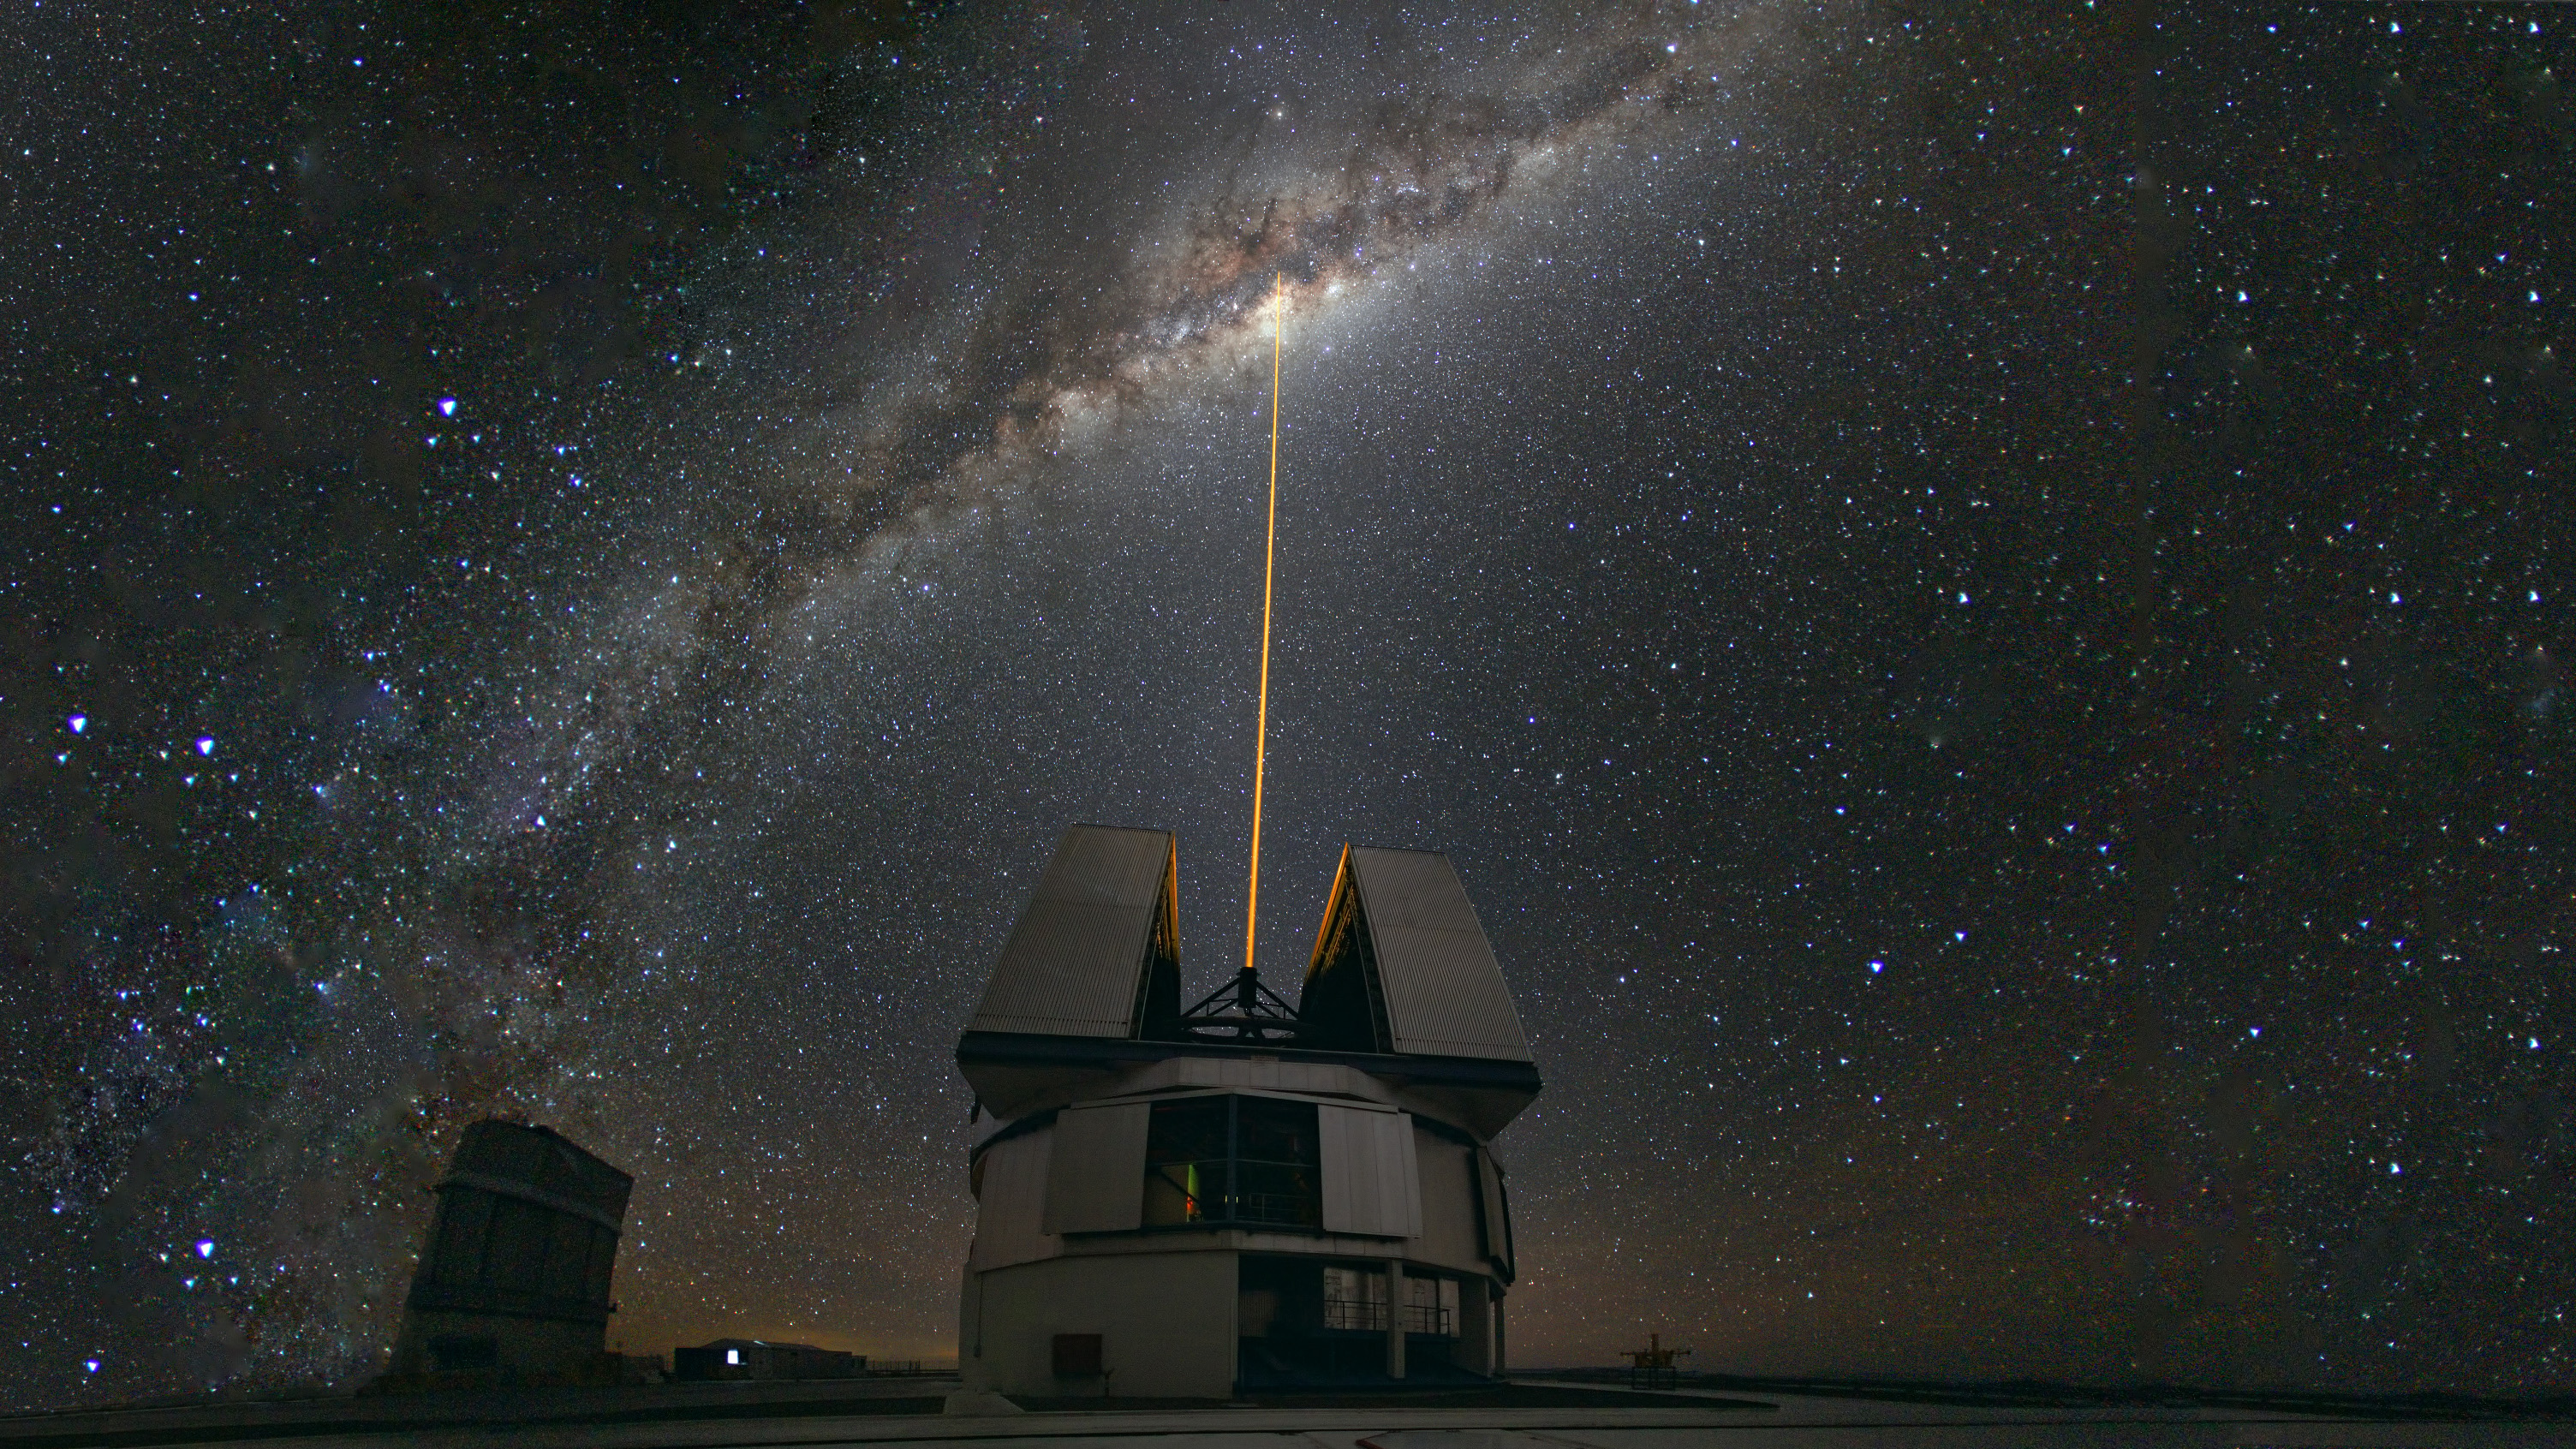
\includegraphics[width=.8\textwidth]{pics/DesignFrameTest_1}
			\end{lstlisting} 
			Vektorgrafiken, z.\,B. SVG-Dateien, müssen vorher in PDFs umgewandelt werden. 
		\end{column}
		\begin{column}{.475\textwidth}
			\centering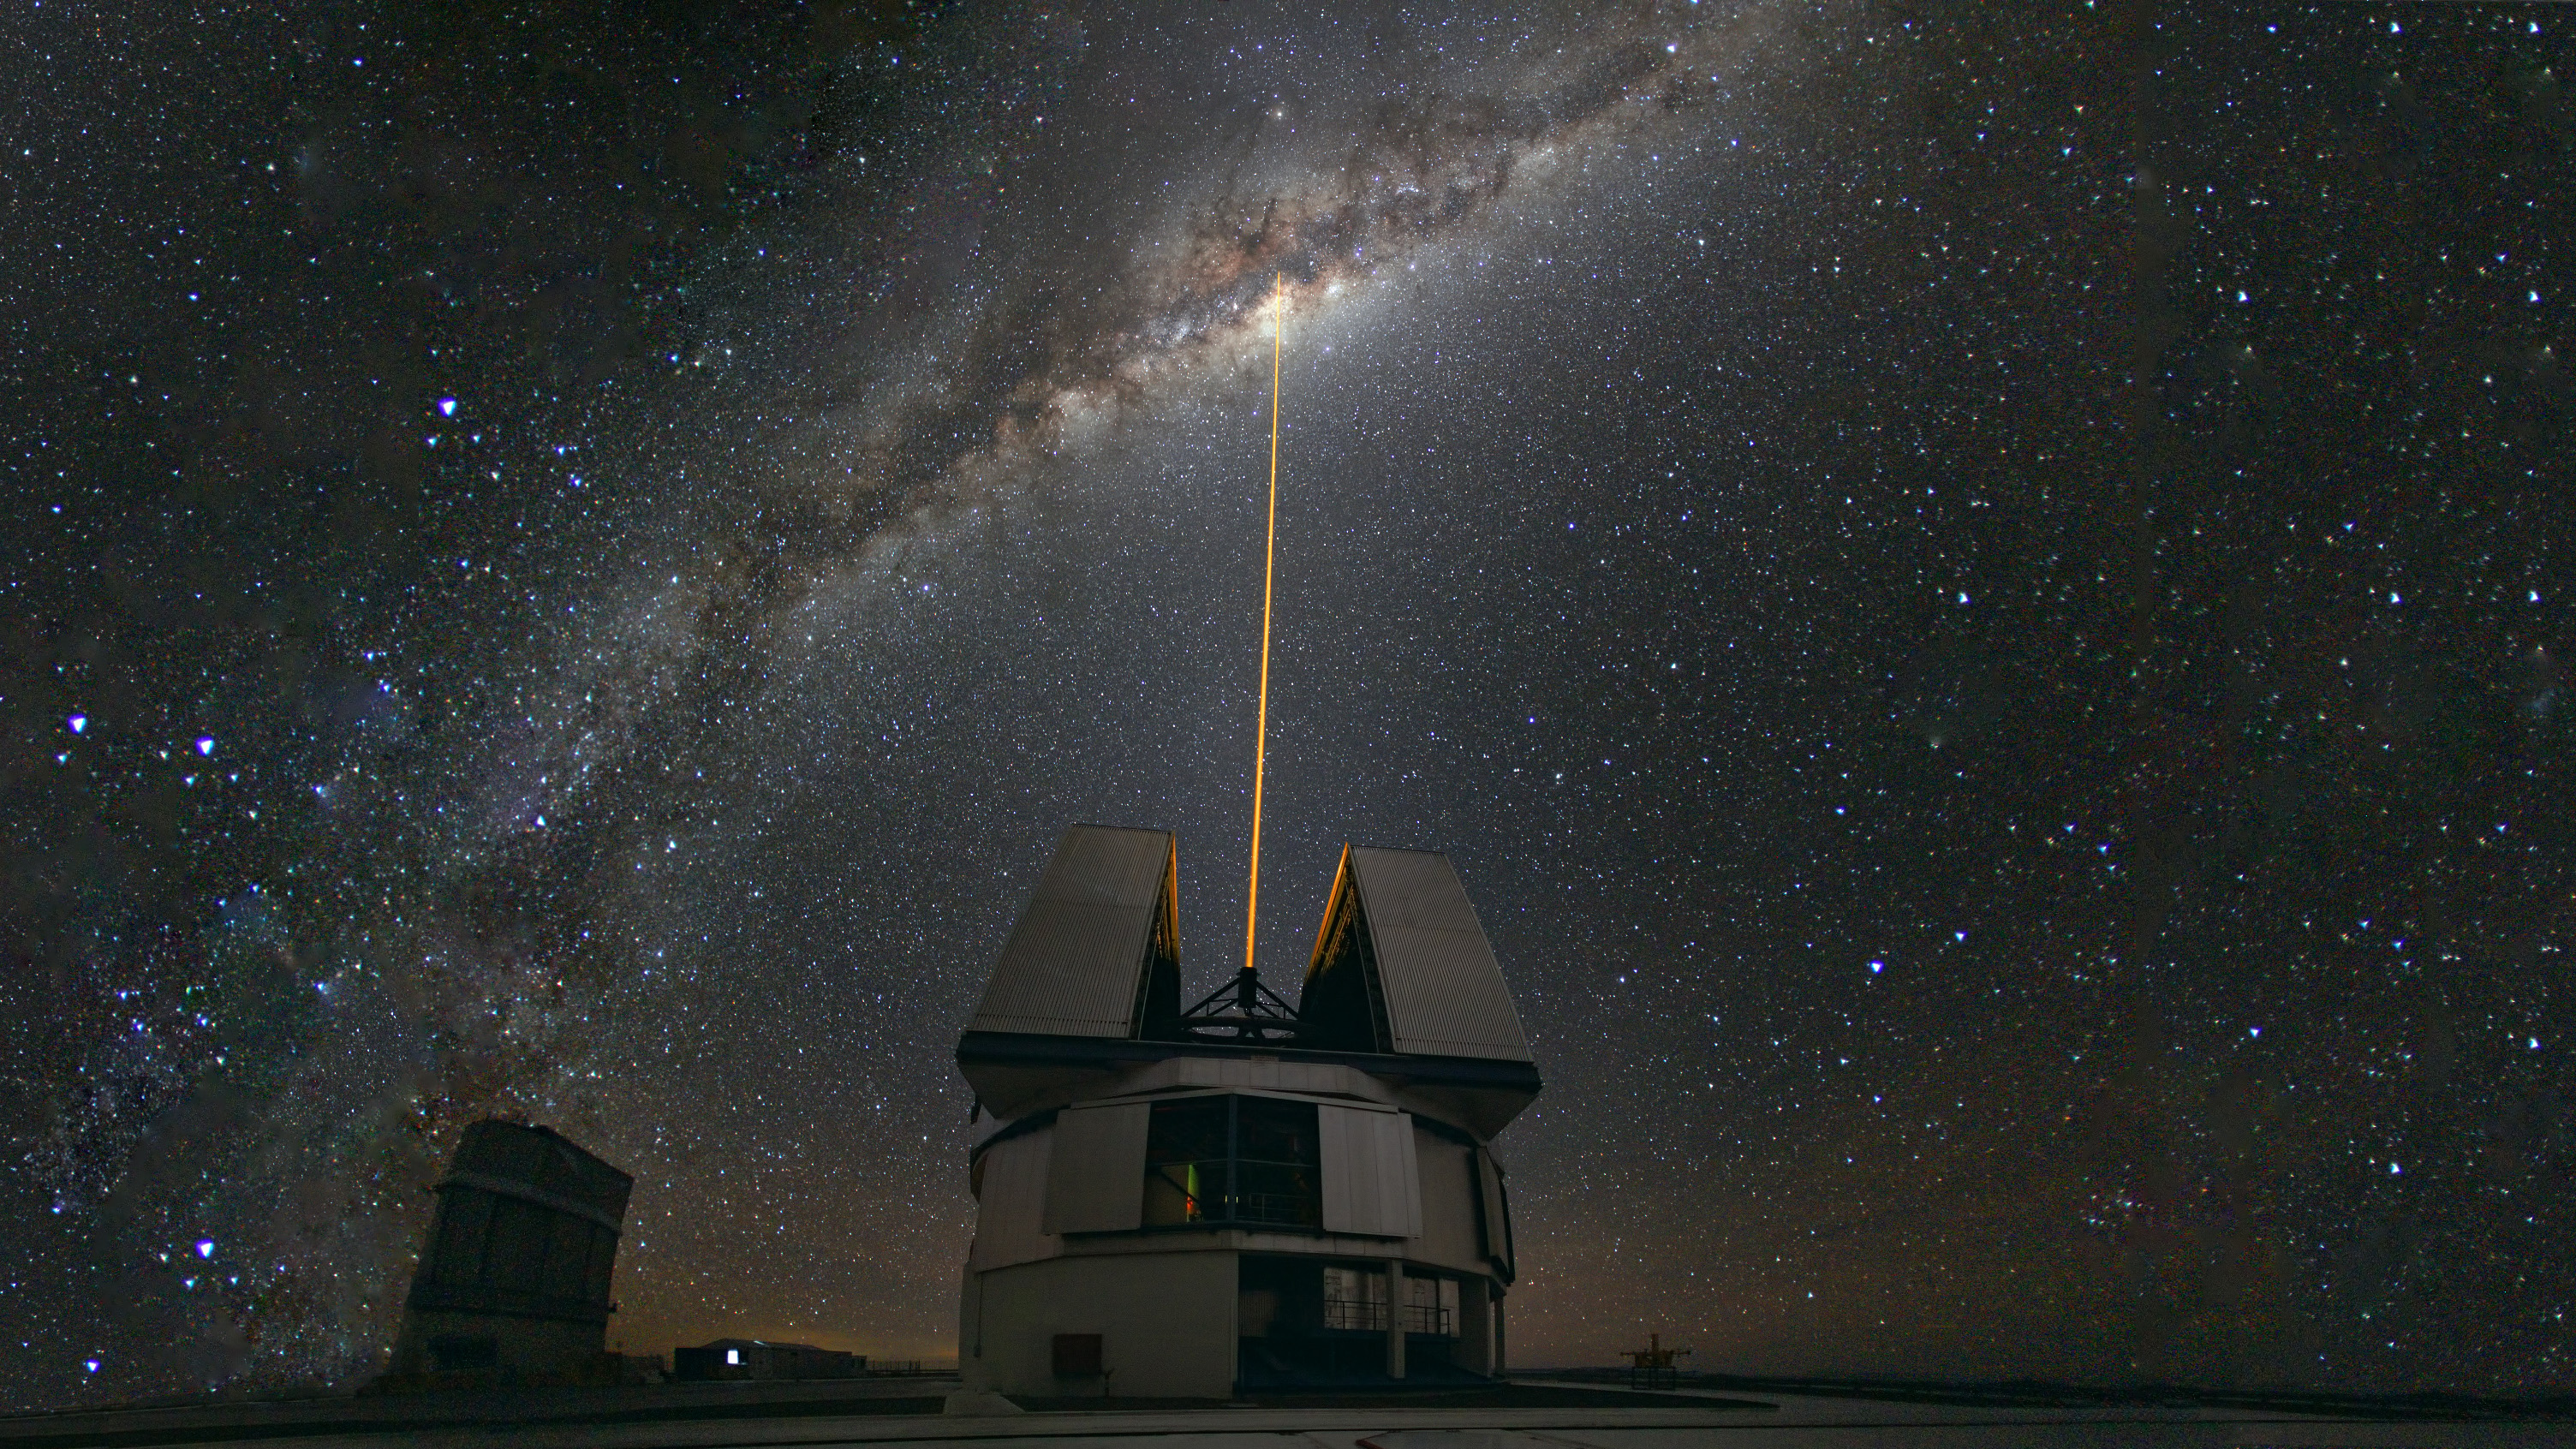
\includegraphics[width=.8\textwidth]{pics/DesignFrameTest_1}
		\end{column}
	\end{columns}
\end{frame}

\begin{frame}[fragile]
	\frametitle{Plots}

	\begin{columns}[T,onlytextwidth]
		\begin{column}{.475\textwidth}
			Die \emph{TikZ}\footnote[frame]{\url{https://www.ctan.org/pkg/pgf}} und \emph{PgfPlots}\footnote[frame]{\url{https://ctan.org/pkg/pgfplots}} Bibliotheken sind bereits in die Klasse eingebunden und können zum Plotten verwendet werden.
			\begin{lstlisting}[gobble=8,style=latex]
				\begin{tikzpicture} 
					\begin{axis}[width = 1\textwidth]
						\addplot3[
							surf,
							samples=15, 
							domain=0:1,
							y domain=-1:1,
							colormap name=tudplot]
							{x^2 - y^2}; 
					\end{axis} 
				\end{tikzpicture}
			\end{lstlisting} 
		\end{column}
		\begin{column}{.475\textwidth}
			\centering%
			\begin{tikzpicture} 
				\ifdraftMode
					\draw (0,0) rectangle (\textwidth,4);
				\else
					\begin{axis}[width = 1\textwidth]
						\addplot3[
							surf,
							samples=15, 
							domain=0:1,
							y domain=-1:1,
					  		colormap name=tudplot]
							{x^2 - y^2}; 
					\end{axis} 
				\fi
			\end{tikzpicture}
		\end{column}
	\end{columns}
\end{frame}

\begin{frame}[fragile]
	\frametitle{Diagramme}

	\begin{columns}[T,onlytextwidth]
		\begin{column}{.475\textwidth}
			Diagramme können ebenfalls mit TikZ erstellt werden, hier ein Beispiel für ein Piechart:
			\begin{lstlisting}[gobble=8,style=latex]
				 % in die Prämbel einfügen
				\usepackage{pgf-pie}
				...
				\adjustbox{max width=\textwidth}{
					\begin{tikzpicture}[]
						\pie [color={emphcyan!70, 
								emphbrightgreen!60,
								emphcyan!60,emphcyan!20,
								emphpurple!70}]{%
							46.6/Chrome,
							24.6/Internet Explorer,
							20.4/Firefox,
							5.1/Safari,
							3.3/Other}
					\end{tikzpicture}
				}
			\end{lstlisting} 
		\end{column}
		\begin{column}{.475\textwidth}
			\adjustbox{max width=\textwidth}{
				\begin{tikzpicture}[]
					\ifdraftMode
						\draw (0,0) rectangle (\textwidth,4);

					\else
						\pie [color={emphcyan!70, emphbrightgreen!60, emphcyan!60, emphcyan!20, emphpurple!70}]{%
							46.6/Chrome,
							24.6/Internet Explorer,
							20.4/Firefox,
							5.1/Safari,
							3.3/Other}
					\fi
				\end{tikzpicture}
			}
		\end{column}
	\end{columns}
\end{frame}

\begin{frame}[fragile]
	\frametitle{Listings}

	\begin{columns}[T,onlytextwidth]
		\begin{column}{.475\textwidth}
			Quellcode-Listings\footnote[frame]{\url{https://www.ctan.org/tex-archive/macros/latex/contrib/listings/}}, können wie folgt eingefügt werden:
			\begin{lstlisting}[gobble=8,style=latex,mathescape]
				\begin{*nframe*}[fragile]
					\begin{*nlstlisting*}[style=latex]
						eine Zeile \LaTeX-Code
						\begin{*nitemize*}
							\item ein Aufzählungsitem
						\end{*nitemize*}
					\ end{*nlstlisting*}
					%Leerzeichen nach \ muss weg
				\end{*nframe*}
			\end{lstlisting}
			Dazu kann der \texttt{latex}-Stil aus der Präambel dieses Dokuments übernommen werden.

			Der Frame muss zwingend auf \texttt{fragile} gesetzt werden.
		\end{column}
		\begin{column}{.475\textwidth}			
			\begin{lstlisting}[gobble=8,style=latex]
				eine Zeile \LaTeX-Code
				\begin{*nitemize*}
					\item ein Aufzählungsitem
				\end{*nitemize*}
			\end{lstlisting}
		\end{column}
	\end{columns}
\end{frame}

\begin{frame}[fragile]
	\frametitle{Tabellen}
	Für Tabellen sind die Pakete \emph{tabularx}\footnote[frame]{\url{https://ctan.org/pkg/tabularx}} und \emph{array}\footnote[frame]{\url{https://ctan.org/pkg/array}} bereits eingebunden.
	\vskip-2ex\begin{columns}[t]
		\begin{column}{.67\textwidth}	
		\begin{lstlisting}[gobble=6,style=latex]
			\begin{table}
			\begin{tabularx}{\textwidth}
				{@{} p{.33\textwidth} p{.33\textwidth} p{.33\textwidth} @{}}
				\hline%
				\textbf{*sAnwendung*}*n&*\textbf{*sPlattform*}*n&*\textbf{*sInhalt*}*n\\*
				\hline%
				Bedienpanel *n&* stationär, TouchPanel *n&* interaktiv*n\\*
				Detailmonitor *n&* stationär, Display *n&* fix*n\\*
				Operatorstation *n&* stationär, PC *n&* interaktiv*n\\*
				\hline%
			\end{tabularx}\caption{*sUIs in Anlagen*}
			\end{table}
		\end{lstlisting}
		\end{column}
	   	\hspace*{-.05\textwidth}\begin{column}{.32\textwidth}
			\begin{table}\begin{tabularx}{\textwidth}{@{} p{.3\textwidth} p{.23\textwidth} p{.2\textwidth} @{}}
			\hline%
			\textbf{Anwendung} & \textbf{Plattform} & \textbf{Inhalt} \\
			\hline%
			Bedien\-panel & stationär, Touchpanel & interaktiv \\
			Detail\-monitor & stationär, Display & fix \\
			Operator\-station & stationär, PC & interaktiv \\
			\hline%
			\end{tabularx}\caption{UIs in Anlagen}\end{table}
		\end{column}
	\end{columns}
\end{frame}
\begin{frame}[fragile]
	\frametitle{Formeln}

	\begin{columns}[T,onlytextwidth]
		\begin{column}[T]{.7\textwidth}
			Formeln können mit Hilfe der \emph{math}-Umgebungen eingefügt werden:
			\begin{lstlisting}[gobble=8,style=latex]				
				\DeclareMathOperator{\Div}{div} % in der Präambel
				\DeclareMathOperator{\Rot}{rot}

				\begin{*nalign*} % in der Folie
					\label{1}
					\Rot\vec{E} &=-\frac{1}{c}\frac{\partial{\vec{B}}}{\partial t}\\
					\label{2}
					\Div\vec{B} &=0\\
					\label{3}
					\Rot\vec{B} &=\frac{1}{c}\frac{\partial {\vec{E}}}{\partial {t}}+\frac{4\pi}{c}\,\vec{j}\\
					\label{4}
					\Div\vec{E} &=4\pi\rho_{\varepsilon}
				\end{*nalign*}
			\end{lstlisting} 
		\end{column}
		\begin{column}[T]{.295\textwidth}
			Die Maxwell'schen Gleichungen:
			\normalsize
			\begin{align}
				\label{1}
				\Rot\vec{E} &=-\frac{1}{c}\frac{\partial{\vec{B}}}{\partial t}
				\\
				\label{2}
				\Div\vec{B} &=0
				\\
				\label{3}
				\Rot\vec{B} &=\frac{1}{c}\frac{\partial {\vec{E}}}{\partial {t}}+\frac{4\pi}{c}\,\vec{j}
				\\
				\label{4}
				\Div\vec{E} &=4\pi\rho_{\varepsilon}
			\end{align}
		\end{column}
	\end{columns}
\end{frame}
\begin{frame}[fragile]
	\frametitle{Blöcke 1}

	\begin{columns}[T,onlytextwidth]
		\begin{column}[T]{.475\textwidth}
			Das Hervorheben wichtiger Elemente und Aussagen ist mit den Block-Umgebungen möglich.
			\begin{lstlisting}[gobble=8,style=latex]			
				\begin{*nblock*}{*sEin Block*}
					Ein Block mit einer wichtigen Aussage.
				\end{*nblock*}
				\begin{*nalertblock*}{*sEin Alertblock*}
					Ein Block mit einer wichtigen Aussage.
				\end{*nalertblock*}
				\begin{*ntheorem*}[*sTesttheorem*]
					Ein Satz. Es gibt auch die Umgebungen \texttt{corollary}, \texttt{fact}, \texttt{lemma}
				\end{*ntheorem*}
				\begin{*nproof*}[*sTestproof*]
					Ein Beweis.
				\end{*nproof*}
			\end{lstlisting} 
		\end{column}
		\begin{column}[T]{.475\textwidth}
			\begin{block}{Ein Block}
				Ein Block mit einer wichtigen Aussage.
			\end{block}
			\begin{alertblock}{Ein Alertblock}
				Ein Block mit einer wichtigen Aussage.
			\end{alertblock}
			\begin{theorem}[Testtheorem]
				Ein Satz. Es gibt auch die Umgebungen \texttt{corollary}, \texttt{fact}, \texttt{lemma}
			\end{theorem}
			\begin{proof}[Testproof]
				Ein Beweis.
			\end{proof}
		\end{column}
	\end{columns}
\end{frame}
\begin{frame}[fragile]
	\frametitle{Blöcke 2}

	\begin{columns}[T,onlytextwidth]
		\begin{column}[T]{.475\textwidth}
			\begin{lstlisting}[gobble=8,style=latex]
				\begin{*nexample*}[*sTestexample*]
					Ein Beispiel.
				\end{*nexample*}
				\begin{*nexampleblock*}{*sTestexampleblock*}
					Ein Beispiel.
				\end{*nexampleblock*}
				\begin{*ndefinition*}[*sTestdefinition*]
					Eine Definition.
				\end{*ndefinition*}
			\end{lstlisting} 
		\end{column}
		\begin{column}[T]{.475\textwidth}
			\begin{example}[Testexample]
				Ein Beispiel.
			\end{example}
			\begin{exampleblock}{Testexampleblock}
				Ein Beispiel.
			\end{exampleblock}
			\begin{definition}[Testdefinition]
				Eine Definition.
			\end{definition}
		\end{column}
	\end{columns}
\end{frame}
\begin{frame}[fragile]
	\frametitle{Textauszeichnung}

	\begin{columns}[T,onlytextwidth]
		\begin{column}{.475\textwidth}
			Weitere Textauszeichnung:
			\begin{lstlisting}[gobble=8,style=latex]
				\begin{*nquote*}
					Quoted Text
				\end{*nquote*}
				\begin{*nquotation*}
					Quotation im Environment
				\end{*nquotation*}
				\begin{*nverse*}
					Ein Vers.
				\end{*nverse*}

				\emph{hervorgehobener Text}\\
				\texttt{inline Quelltext}\\
				\alert{alarmierender Text}\\
				\url{*shttp://tu-dresden.de*}
			\end{lstlisting} 
		\end{column}
		\begin{column}{.475\textwidth}
			\begin{quote}
				Quoted Text
			\end{quote}
			\begin{quotation}
				Quotation im Environment
			\end{quotation}
			\begin{verse}
				Ein Vers.
			\end{verse}

			\emph{hervorgehobener Text}\\
			\texttt{inline Quelltext}\\
			\alert{alarmierender Text}\\
			Eine URL: \url{http://tu-dresden.de}
		\end{column}
	\end{columns}
\end{frame}

\begin{frame}[fragile,label=buttonsnfootnotes]
	\frametitle{Buttons und Fußnoten}

	\begin{columns}[T,onlytextwidth]
		\begin{column}{.475\textwidth}
			Wenn Frames mit einem label versehen werden, können Links bzw. Beamer-Buttons verwendet werden, um dorthin zu navigieren:
			\begin{lstlisting}[gobble=8,style=latex,numbers=none]				
				\begin{*nframe*}[label=*sbuttonsnfootnotes*]
			\end{lstlisting}
			Ein Button kann wie folgt eingebaut werden:
			\begin{lstlisting}[gobble=8,style=latex,numbers=none]
				\hyperlink{movies}{\beamergotobutton{Movies}}
			\end{lstlisting}
			Ein Button zu einer Webseite:
			\begin{lstlisting}[gobble=8,style=latex,numbers=none]
				\hyperlink{http://tu-dresden.de}{\beamergotobutton{TU-Dresden Homepage}}
			\end{lstlisting}
		\end{column}
		\hspace{.05\textwidth}\begin{column}{.475\textwidth}
			Der Button zu der Movie-Folie: \hyperlink{movies}{\beamergotobutton{Movies}}\\
			Der Button zu einer Webseite: \hyperlink{http://tu-dresden.de}{\beamergotobutton{TU-Dresden Homepage}}\\
			\vskip6ex
			Fußnoten sind für Präsentationen i.\,d.\,R. nicht geeignet und sollten nur verwendet werden, wenn ein Handout oder eine digitale Kopie bereitgestellt wird.			
			\begin{lstlisting}[gobble=8,style=latex,numbers=none]
				Text in einer Column\footnote{engl. für Spalte}-Umgebung\footnote[frame]{Fußnote am Frameende}.
			\end{lstlisting}
			\vskip2ex
			Das Ergebnis:\\
			Text in einer Column\footnote{engl. für Spalte}-Umgebung\footnote[frame]{Fußnote am Frameende}.
		\end{column}
	\end{columns}
\end{frame}
\begin{frame}[fragile,label=movies]
	\frametitle{Movies}

	\begin{columns}[T,onlytextwidth]
		\begin{column}{.475\textwidth}
			Das Einbinden von Videos\footnote[frame]{per \emph{multimedia}-Package} ist zwar möglich, das Ergebnis hängt allerdings sehr vom verwendeten PDF-Viewer ab.
			\begin{lstlisting}[gobble=8,style=latex]
				\movie%
					[label=space,width=\textwidth,externalviewer]{%
						\includegraphics%
							[width=1\textwidth]%
							{*spics/movie-backup*}%
					}%
					{*spics/the-space-shuttle-rocket-launch.mp4*}
			\end{lstlisting}
			Daher sollte die Option \texttt{externalviewer} verwendet werden.
		\end{column}
		\begin{column}{.475\textwidth}
		\movie[label=space,width=\textwidth,externalviewer]{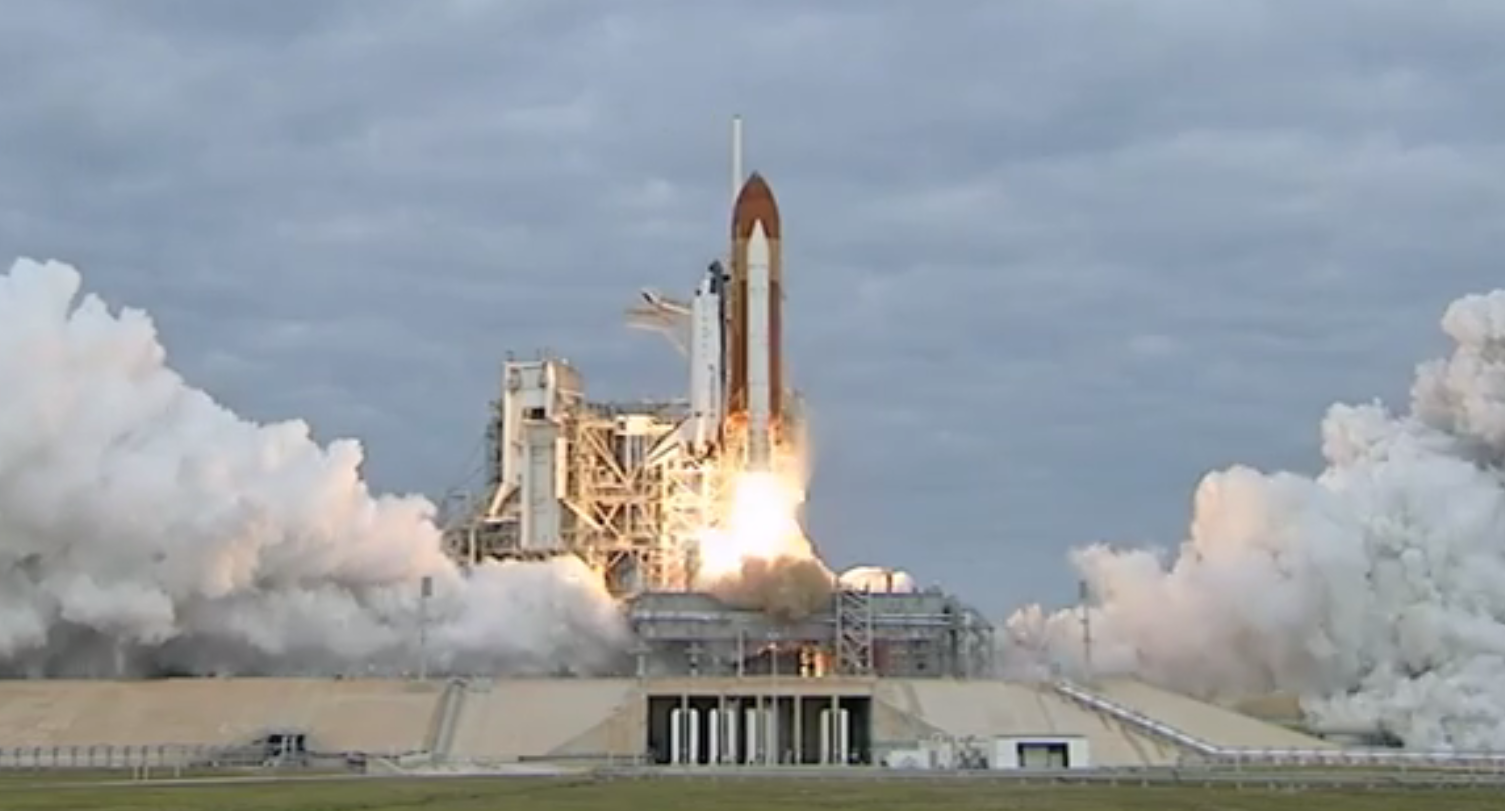
\includegraphics[width=1\textwidth]{pics/movie-backup}}{pics/the-space-shuttle-rocket-launch.mp4}\\
		{\tiny Quelle: \url{https://www.youtube.com/watch?v=m8d2Lxefb3c}, CC0-Lizenz}
		\end{column}
	\end{columns}

	Zurück zu \hyperlink{buttonsnfootnotes}{\beamergotobutton{Buttons und Fußnoten}}.
\end{frame}

\subsection{Animationen}
\begin{frame}[fragile]
	\frametitle{Animationen}

	Die allermeisten Inhalte einer Folie können durch Overlay-Spezifikationen animiert werden. Dabei erstellt die Beamer-Klasse mehrere aufeinander folgende Seiten im PDF für dieselbe Folie.

	\begin{columns}[T,onlytextwidth]
		\begin{column}{.5\textwidth}					
			Beispiel:
			\begin{lstlisting}[gobble=8,style=latex]
				\begin{*nitemize*}
					\item<1-> \color<1>{emphblue}Dieses Item ist ab dem ersten Overlay vorhanden, aber nur auf dem ersten blau
					\item<2-3> Dieses Item auf den Overlays 2 und 3
					\item<-2> Dieses Item auf den Overlays 1 und 2
					\item<handout> Dies Item befindet sich nur auf dem Handout
				\end{*nitemize*}
			\end{lstlisting}
		\end{column}
		\begin{column}{.4\textwidth}				
			\begin{itemize}
				\item<1-> \color<1>{emphblue}Dieses Item ist ab dem ersten Overlay vorhanden, aber nur auf dem ersten blau
				\item<2-3> Dieses Item auf den Overlays 2 und 3
				\item<-2> Dieses Item auf den Overlays 1 und 2
				\item<handout> Dieses Item befindet sich nur auf dem Handout
			\end{itemize}
		\end{column}
	\end{columns}
\end{frame}
\begin{frame}[fragile]
	\frametitle{Grafiken animieren}

	\begin{itemize}
		\item Die Befehle \texttt{\textbackslash uncover<>\{\}}, \texttt{\textbackslash only<>\{\}}, etc. funktionieren auch in Tabellen und \texttt{tikzpicture}-Umgebungen. Somit lassen sich Grafiken animieren.
		\item Wird ein Grafikprogramm verwendet muss man u.\,U. die Grafik mehrfach zeichnen und verschiedene Versionen per Overlay einbinden.
		\item Für Visio-Grafiken steht dafür ein Export-Skript zur Verfügung. 
	\end{itemize}

	\begin{columns}[T,onlytextwidth]
		\begin{column}{.5\textwidth}					
			Beispiel:
			\begin{lstlisting}[gobble=8,style=latex]			
				\includegraphics<1>[width=\textwidth]{*spics/Animation0*}%	
				\includegraphics<2>[width=\textwidth]{*spics/Animation1*}%	
				\includegraphics<3>[width=\textwidth]{*spics/Animation2*}%	
			\end{lstlisting}
			Wichtig ist das \%-Zeichen am Ende der Include-Anweiseung.
		\end{column}
		\begin{column}{.4\textwidth}	
			\includegraphics<1>[width=\textwidth,trim=4 4 4 4,clip]{pics/Animation0}%	
			\includegraphics<2>[width=\textwidth,trim=4 4 4 4,clip]{pics/Animation1}%	
			\includegraphics<3>[width=\textwidth,trim=4 4 4 4,clip]{pics/Animation2}%	
		\end{column}
	\end{columns}
\end{frame}

\section{Weitere Tipps}
\subsection{Git}

\begin{frame}
	\frametitle{Latex und Git}
	\begin{itemize}
		\item Da LaTeX hauptsächlich auf reinen Textdateien basiert, eignen sich die Quelldateien für die Versionierung, z.\,B. mit Git.
		\item Damit Änderungen jeweils optimal nachverfolgt werden können, sollte die Zeichenanzahl pro Zeile in der Quelldatei begrenzt werden. Einige Editoren bieten dazu ein \emph{Word-Wrap}-Feature an.
		\item Die Temporären LaTeX-Dateien sollten nicht eingecheckt werden, die erzeugten PDFs ebenso nicht.
		\item Das Klassenprojekt enthält für Git eine \emph{.gitignore}-Datei, die in das eigene LaTeX-Projekt kopiert werden kann.
	\end{itemize}
\end{frame}

\section{Verschiedene Tests}	
\subsection{Designfolien}

\begin{frame}
	\frametitle{Designfolien}
	\framesubtitle{TODO}
\end{frame}

%\subsection{Sonstiges}

\subsection{Debug}
\makeatletter
\begin{frame}[allowframebreaks]
	\frametitle{Debug}
	sizes:
	\begin{enumerate}
		\item beamerwidth : \the\paperwidth, beamerheight: \the\paperheight
		\item beamerwidth : \number\paperwidth, beamerheight:\number\paperheight
		\item body: \the\bodyx, \the\bodyy; \the\bodywidth, \the\bodywidth
		\item author: \insertauthor
		\item title: \inserttitle
		\item subtitle: \insertsubtitle
		\item datecity: \insertdatecity
		\item fsize: \f@size
	\end{enumerate}
\end{frame}
\makeatother

%
% Backmatter
%
%%%%%%%%%%%%%%%%%%%%%%%%%%%%%%%%%%%%%%%%%%%%%%%%%%%%%%%%%%%%%%%%%%%%%%%%%%%%%%%%%%%%%%%%%%%%%%%%%%%%%%%%%%%%%%%%%%%%%%%%%%%%%

\disableSectionFrame%
%\disableFrameTitleSectionNum%
\section*{Backmatter}
\begin{finalframe}
	\vskip4ex\begin{columns}
	    \begin{column}{0.5\textwidth}        
	        \huge Vielen Dank\\ für Ihre Aufmerksamkeit\\[1ex]\
	    \end{column}
	    
	    \begin{column}{0.3\textwidth}
	        \flushright{
\includegraphics[keepaspectratio=true,width=.6\columnwidth]{IfA_logo_weiss}}
        	\vspace{1ex}\\

	        \large Lukas Baron\\[0.5ex]
	        \scriptsize
	        lukas.baron@tu-dresden.de\\[4ex]
        	Dresden, Germany\\[4ex]\
	    \end{column}
	\end{columns}
\end{finalframe}

\begin{finalframe}
	\vspace*{2ex}\centering
\includegraphics[width=0.8\textwidth]{br_logo_weiss.png}
\end{finalframe}

% \begin{frame}
% 	\frametitle{test}
% 	test
% \end{frame}

% % additional pages for Q&A purposes
\begin{backmatterframe}
	\frametitle*{Feedback}
	\centering\Huge ? \scriptsize
	\vskip4ex
		Bei Fragen, Problemen uns Verbesserungen,\\ kann der Issue-Tracker\\ im 
		\href{%
			https://git.agtele.eats.et.tu-dresden.de/agtele-public/latex/de.tud.et.ifa.latex.ifaslides/issues%
		}{%
			\beamergotobutton{AG-Tele GitLab%
				\footnote[frame]{\url{https://git.agtele.eats.et.tu-dresden.de/agtele-public/latex/de.tud.et.ifa.latex.ifaslides/issues}}%
			}%
		}
		verwendet werden.
\end{backmatterframe}

\appendix
\begin{frame}[fragile]
	\frametitle{Appendix}

	\begin{columns}[T,onlytextwidth]
		\begin{column}{.475\textwidth}	
			Ein Appendix kann wie folgt eingefügt werden:	
			\begin{lstlisting}[gobble=8,style=latex]			
			\end{lstlisting}
		\end{column}
		\begin{column}{.475\textwidth}	
		\end{column}
	\end{columns}
\end{frame}

\end{document}
